\chapter[Theory and Experimental Methods]{Theory and Experimental Methods}
\setcitestyle{citesep={,\,\thechapter.}}
\section{EPR spectroscopy}

In this section, the underlying theoretical and practical principles of the EPR experiment will be discussed as it relates to the experiments performed in this work. 

\subsection{Spin Hamiltonian}
The complete Hamiltonian $\mathcal{H}_0$ of a molecular system is very complex. All of the space and spin coordinates of electrons and nuclei would be included in the complete Hamiltonian, such that,
\begin{equation}
    \mathcal{H}_0 \ket{\Psi} = {\mathbf E} \ket{\Psi}
\end{equation}
where the wave function $\ket{\Psi}$ describes how the molecular system is propagated over time, known as the time-dependant Schr\"{o}dinger equation. Since EPR measures the time-invariant ground states, it is sufficient to describe only the interactions of the molecular system energy contained in the Hamiltonian. The energy states ${\mathbf E}$ are further simplified by the phenomenologically derived spin Hamiltonian operator $\hat{\mathcal{H}}$ and the time-dependant Schr\"{o}dinger equation is simplified to only the spin states of the system. \cite{SpinDyn,abragam1961} 

The spin Hamiltonian comprises of the superposition of the magnetic and electric properties of the molecular system, such that,
\begin{equation}
    \hat{\mathcal{H}} = \hat{\mathcal{H}}_{ze} + \hat{\mathcal{H}}_{hfi} + \hat{\mathcal{H}}_{nz} + \hat{\mathcal{H}}_{nqi} + \hat{\mathcal{H}}_{zfs},
\end{equation}
where the electron Zeeman interaction $\hat{\mathcal{H}}_{ze}$, the hyperfine interaction $\hat{\mathcal{H}}_{hfi}$, the nuclear Zeeman interaction $\hat{\mathcal{H}}_{nz}$, and, for nuclei with $I > 1/2$, the electric-nuclear quadrupole interactions $\hat{\mathcal{H}}_{nqi}$. The zero-field splitting term $ \hat{\mathcal{H}}_{zfs}$, is characterized by an electron-spin magnetization without an applied static magnetic field. 

\begin{figure}[ht]
 \centering
 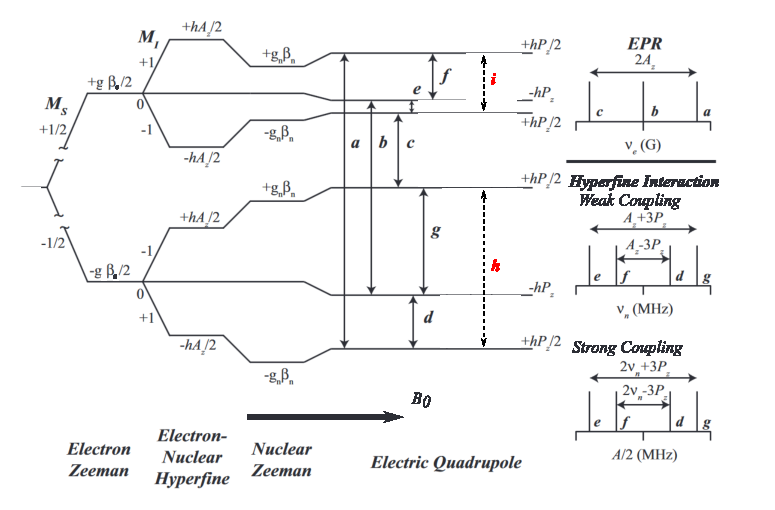
\includegraphics[width=\textwidth]{Kapitel/Ch2-Images/EnergyDiagram.eps}
 \caption[Energy diagram example with S=1/2 and I=1.]{Energy diagram example of a spin system with $S=1/2$, $I=1$, and first-order quadrupole interactions. The transitions $\mathbf{a}$, $\mathbf{b}$, and $\mathbf{c}$ are EPR transitions. The nuclear hyperfine-interaction transitions are marked as $\mathbf{d}$, $\mathbf{e}$, $\mathbf{f}$, and $\mathbf{g}$. The transitions shown as dashed lines are semi-forbidden ``double quantum'' $\Delta M_I = \pm 2$ transitions and marked in red as marked as $\mathbf{h}$ and $\mathbf{i}$. Modified with permission from Fig.~2 of Ref.~[2.\kern-0.4em\citenum{CUTSAIL20151370}].}
 \label{fig:EPREnergy}
\end{figure}

In this formulation, the static magnetic field $\mathbf{B}_0$ is assumed to be along the $z$ axis and denote the transpose of a tensor with a `T'. In this work, it is assumed that the electron Zeeman interaction is the largest interaction followed by the hyperfine interaction, nuclear Zeeman, electric quadrupole, and zero-field splitting.

\subsubsection*{Zeeman interactions}
When a static magnetic field is applied to a molecular system with angular momentum, the angular momentum aligns in such a way that a Boltzmann distribution is formed. This removes the degeneracy of the electron magnetization $\mathbf{M}_s$ manifold, splitting the energy levels, illustrated in Fig.~\ref{fig:EPREnergy} as the initial splitting. For an electron spin of $S = 1/2$, the initial energy levels are split into $\mathbf{M}_s = \ket{+\frac{1}{2}}, \ket{-\frac{1}{2}}$ for spin-up and spin-down, respectively. Both the electron $\hat{\mathcal{H}}_{ze}$ and nuclear $\hat{\mathcal{H}}_{nz}$ Zeeman interactions occur when a static magnetic field $\mathbf{B}_z$ is applied.

The electron Zeeman interaction is defined by
\begin{equation*}
    \hat{\mathcal{H}}_{ze} = \beta_e \mathbf{B}^\text{T}_z  \cdot \mathbf{g} \cdot \mathbf{S}
\end{equation*}
where $\beta_e$ is the Bohr magneton, the transpose of the static magnetic field $\mathbf{B}_z^{\text{T}}$, the vector operator $\mathbf{S} = [\mathbf{S}_x \; \mathbf{S}_y \; \mathbf{S}_z]$ is the spin angular momentum of the electron. 

A free electron in a vacuum has an isotropic spin with angular momentum. It is then the introduction of the electron with other atoms and how those atoms distribute the electron that gives rise to different components of the spin Hamiltonian.\cite{abragam2012electron,harriman1978theoretical} This ``pushing'' and ``pulling'' of the electron by spin-orbit coupling leads to anisotropic $\mathbf{g}$. The matrix $\mathbf{g}$ is what is known as the $g$-tensor and is a spatial distribution of the angular momentum of the electron. The $g$-tensor is typically made diagonal and discussed in terms of the $g_x$, $g_y$, and $g_z$ principal components, where the magnitude is denoted as $g_{iso}$. EPR resonance occurs as a result of the incident energy is matched by the energy difference of the electron Zeeman levels. 

Deviations from a free-electron can be used to obtain information on the local environment. Since these processes are non-cooperative, we can separate the free-electron from all the other contributions
\begin{equation*}
    \mathbf{g} = g_e \mathbf{1} + \Delta \mathbf{g},
\end{equation*}
where $\mathbf{1}$ is the identity matrix and $\Delta \mathbf{g}$ includes isotropic terms as well as second-order spin-orbit coupling terms. The interaction between the electron spin and the atomic orbitals of the molecule arise due to the magnetic moment of the electron. \cite{griffith1964theory} The electron Zeeman $\hat{\mathcal{H}}_{ze}$ interaction is then a perturbation of the free electron in the ground state. 

For systems when the electron interacts with intrinsic or surrounding nuclei with a nuclear spin $I_k$, the Nuclear Zeeman effect is added to $\hat{\mathcal{H}}$ as
\begin{equation*}
    \hat{\mathcal{H}}_{nz} = - \beta_n \sum_{k=1}^m g_{n,k} \mathbf{B}^\text{T}_z  \cdot \mathbf{I}_k,
\end{equation*}
where $\beta_n$ is the nuclear magneton, the transpose of the static magnetic field $\mathbf{B}_z$ is marked with a `T', the vector operator $\mathbf{I}_k = [\mathbf{I}_x \; \mathbf{I}_y \; \mathbf{I}_z]$ is the spin angular momentum of the nuclei. The summation of the nuclear contributions are represented by the index $k$ for each $m$ nucleus that interacts with the electron. Each nucleus has a distinct nuclear $g_{n,k}$-value and angular momentum $\mathbf{I}_k$ and is assumed to be isotropic. The visualization of the nuclear Zeeman effect is illustrated as a perturbation on the electron-nuclear hyperfine interaction shown in Fig.~\ref{fig:EPREnergy}.

\subsubsection*{Nuclear-Electron Interactions}
Since EPR is the measurement of how a valence electron interacts with the surrounding environment, information on the surrounding nuclei is possible if these nuclei have an inherent nuclear spin $\mathbf{I}$. Such nuclei include, for example, $^1$H, $^2$H, $^{14}$N, $^{15}$N, $^{57}$Fe, and $^{13}$C, which can be synthetically incorporated into the system to gain more information than the natural abundance of some of the atoms. \cite{Doorslaer2007,Harmer2009,CUTSAIL20151370}

\paragraph*{Hyperfine Interactions}
The hyperfine interactions are defined as the coupling between the paramagnetic site and the surrounding nuclei. This can be broken up into two distinct parts, the isotropic Fermi contact interaction, $a_{iso}$, and the electron-nucleus magnetic dipole-dipole coupling. The hyperfine interactions can be expressed as
\begin{equation}
    \hat{\mathcal{H}}_{hfi} = \mathbf{S}^{\text{T}} \cdot \mathbf{A} \cdot \mathbf{I}_k = a_{iso}\mathbf{S}^{\text{T}} \cdot \mathbf{I}_k + \mathbf{S}^{\text{T}} \cdot \mathbf{T} \cdot \mathbf{I}_k \label{eq-2:hfi}
\end{equation}
for each the interacting nuclei $k$, there exists such an interaction. The Fermi contact describes the delocalization of the electron to the surrounding nuclei. At a sufficient distance, the spacial tensor $\mathbf{T}$ can be described by
\begin{equation}
    \mathbf{T} = \frac{\mu_0}{4 \pi \hbar}\frac{1}{r^3} g_n \beta_n \beta_e g_i (3r_i r_j - \delta_{ij}) \qquad (i,j = x,y,z), \label{eq-2:hfiT}
\end{equation}
where the $x$, $y$, and $z$-components of the hyperfine tensor are treated independently. Illustrated in Fig.~\ref{fig:EPREnergy} is the nuclear-electron hyperfine interaction assuming only the isotropic component of interaction. In frozen solution, this isotropic component is broadened by the distribution of the frequency components defined by $\mathbf{T}$. Only single-crystal EPR spectroscopy can truly obtain the full hyperfine-tensor information for systems with anisotropic hyperfine interactions $\mathbf{T}$ by measuring the total hyperfine interaction $\mathbf{A}$.

\paragraph*{Electric-Nuclear Quadrupole Interactions}
The electric-nuclear quadrupole interaction only exists for nuclei with a spin $I$ greater than 1/2 and is caused by electric field gradients due to the interaction of the electron with the second moment of the nuclear angular momentum. This can be rationalized since the nuclear Zeeman interaction is assumed to be isotropic, while the second moment (gradient) is a measurement of the deviation from isotropic angular momentum. One can learn about the nature of the chemical bonding and the delocalization of the electron if the quadrupole moment $Q$ is known.\cite{quadref} 

The electric-nuclear quadrupole interaction is described by the Hamiltonian
\begin{equation}
    \hat{\mathcal{H}}_{nqi} = \mathbf{\hat{I}}^\text{T} \cdot \mathbf{P} \cdot \mathbf{\hat{I}} \label{eq-2:nqi}
\end{equation}
where
\begin{equation}
    \mathbf{P} = P_{||}   \begin{bmatrix}
   \eta_Q -1 & 0 & 0\\
     & \eta_Q -1 & 0\\
    &   & 2\\
   \end{bmatrix}
\end{equation}
and the value 
\begin{equation}
    P_{||} = \frac{3 e Q}{4I(2I-1)}\frac{\partial^2 V}{\partial z^2} = \frac{3 P_z}{2}
\end{equation}
where $\frac{\partial^2 V}{\partial z^2}$ is the electric-field gradient seen by the nucleus and $|e|Q$ describes the electric shape of the nucleus and is directly determined by the type of nucleus and, here, $\eta$ is defined as the rhombicity of the electric gradient calculated by $(Px-Py)/P_z$ when $|P_z|\geq |P_y|\geq |P_x|$. \cite{abragam2012electron,weil2007electron} The final EPR spectrum is a combination of all of these effects yielding a change in the Boltzmann population at the static magnetic field position illustrated in Fig.~\ref{fig:EPREnergy} as arrows marked $\mathbf{a}$, $\mathbf{b}$, and $\mathbf{c}$ and plotted as a transition stick diagram in the top right.

The hyperfine interactions that are measured with some double-resonance experiments are indicated in Fig.~\ref{fig:EPREnergy} as the arrows marked $\mathbf{d}$, $\mathbf{e}$, $\mathbf{f}$, and $\mathbf{g}$. However, when performing hyperfine spectroscopy the semi-forbidden ``double quantum'' (DQ) transitions need to be understood. In Fig.~\ref{fig:EPREnergy}, these transitions are shown as dashed lines and marked in red as $\mathbf{h}$ and $\mathbf{i}$. The DQ transitions are a second-order effect on the electric-nuclear quadrupole interactions and can be calculated by
\begin{equation}
\nu^{DQ}_{\alpha, \beta} = 2 \sqrt{\bigg(\nu_I \pm \frac{a}{2}\bigg)^2+\bigg(\frac{e^2 q Q}{4 h}\bigg)(3+\eta)}, \label{eq-2:doubleQ}
\end{equation}
where $a$ is the hyperfine coupling at the nuclei of interest. \cite{Doorslaer2007} This splitting further complicates the interpretation of the data. However, when measured in single crystals the double-quantum cross peaks can be used to assign nuclei throughout the rotation.

\subsubsection*{Multiple Electron Interactions}
\paragraph*{Zero-field Splitting}
For electron with spin greater than 1/2 ($S > 1/2$) or an effective spin of multiple electrons with strong coupling greater than 1/2 ($S_{eff} > 1/2$), there exists an internal interaction that splits the energy levels of the ground state with no applied external field. This interaction, named zero-field splitting, is defined as 
\begin{equation}
    \hat{\mathcal{H}}_{zfs} = \mathbf{S}^{\text{T} } \cdot \mathbf{D} \cdot \mathbf{S}
\end{equation}
where the zero-field splitting tensor $\mathbf{D}$ is a symmetric interaction from close spin-orbital coupling between two or more electrons. The zero-field splitting is especially important in molecular magnets, where it is the direct characterization of the magnetization caused by the interactions of electrons as magnetic monopoles. \cite{barra1998high} With very large values of $D$, the EPR transistion only become excited with high-field--high-frequency EPR methods. \cite{Nehrkorn13} 

\section{On the use of Magnetic Field and Flux Density}
The EPR literature uses the magnetic field $\mathbf{H}$ and magnetic flux density $\mathbf{B}$ interchangeably as ``magnetic field''. It is somewhat disingenuous to state that the relationship of the magnetic field and magnetic flux density is simply related by the free-space permeability $\mu_0$. The focus of this section is to define the usage in this dissertation by following the nomenclature of Jackson of Ref.~[2.\kern-0.4em\citenum{jackson1975classical}] so that 
\begin{equation}
    \mathbf{B} = \mu_0(\mathbf{M} + \mathbf{H}),
\end{equation}
where the SI units for $\mathbf{B}$ is measured in Tesla, while $\mathbf{H}$ is calculated in Ampere per meter. The magnetic susceptibility $\mathbf{M}$ becomes relevant when the time-varying magnetic flux density $\mathbf{B}$ is incident on a material, such as a sample. For brevity, the time-varying magnetic flux density is defined as
\begin{equation}
    \mathbf{B}_1 = \mathbf{B} e^{-i\omega t}
\end{equation}
where $\omega$ is the frequency of interest (radians per second). It is the magnetic flux density that is incident on the sample defined by the magnetic field profile of the microwave resonator. As anticipated, the magnetic susceptibility is material-specific and is proportional to the magnetic moment of the material. In a macroscopic sense, it is the perturbation of this magnetic moment that is measured in EPR. For experimental methods, this is described in detail in Section~2.5 and used extensively in the formulation of Chapter~4. The magnetic susceptibility has the units of Ampere per meter.

From Maxwell's equations, the magnetic field is calculated by the curl of the magnetic potential and, in a vacuum, describes the relationship of the applied currents to the geometry and boundary conditions. \cite{jackson1975classical} In this dissertation when a microwave resonator is discussed, it is the magnetic field profile that is calculated and plotted. However, it is the magnetic flux density that interacts with the sample and is the experimentally measurable quantity. This is because the magnetic flux density is the mechanical torque that is applied to the magnetic moment of the material. 

This distinction is constant throughout the dissertation. If the quantity is measurable and interacts with the sample, it must be described in terms of the magnetic flux density $\mathbf{B}_1$, while calculated profiles are described in terms of magnetic field $\mathbf{H}_1$.

Finally, the static magnetic field is simply referred to as $\mathbf{B}_0$ with units of miliTesla (10$^{-1}$ Gauss\footnote{In modern EPR literature the use of mT is now favored over G.}) since no time-varying magnetic susceptibility exists. A static magnetic field is the only instance where the dual ``magnetic field'' nomenclature is correct when referring to~$\mathbf{B}$.

\section{Crystal Orientations and Molecular Frames}
In this section, the basic understanding of crystal orientations and how to relate them to the EPR experiment is discussed. 

\begin{figure}[ht]
 \centering
 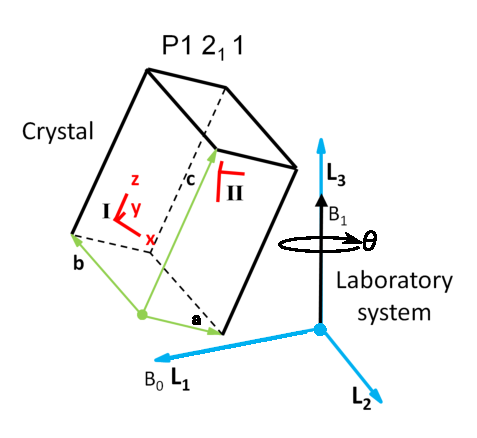
\includegraphics[width=0.75\textwidth]{Kapitel/Ch1-images/CrystalRotation.eps}
 \caption[Single crystal EPR frames.]{Relation of the Laboratory system frame $[\mathbf{L}_1\; \mathbf{L}_2\; \mathbf{L}_3]$ to the crystal frame $[\mathbf{a}\; \mathbf{b}\; \mathbf{c}]$ and the molecular frame $[\mathbf{x}\; \mathbf{y}\; \mathbf{z}]$. The molecular frame at Site I and Site II are related the crystal symmetry. The P$1\;2_1\;1$ crystal symmetry depicted here is occurs in CpI [FeFe]-hydrogenase PDB ID: 4XDC.\cite{FeFeCry} used in Chapter~6.}
 \label{fig:CrystalOrientation}
\end{figure}

\paragraph*{Laboratory System Frame} The Laboratory system frame $[\mathbf{L}_1\; \mathbf{L}_2\; \mathbf{L}_3]$ is illustrated in Fig.~\ref{fig:CrystalOrientation} as the blue coordinate system. The laboratory system frame represents the physical coordinates as it exists in the EPR laboratory. The laboratory system frame is defined with the static magnetic field (${\textbf B}_0$) oriented along the L$_1$-axis, while the microwave magnetic flux density (${\textbf B}_1$) is along the L$_3$-axis. 

\paragraph*{Crystal Frame} The crystal frame $[\mathbf{a}\; \mathbf{b}\; \mathbf{c}]$ is defined with respect to the laboratory frame. When the crystal is inserted into the resonator, the crystal orientation is typically unknown. The crystal frame rotation can be defined by a set of Euler angles. Herein the nomenclature of the EasySpin simulation package. \cite{STOLL200642} The three Euler angles ($\alpha$, $\beta$, $\gamma$) define the rotation around defined axes of the current frame. The first angle $\alpha$ is a rotation around the $z$-component, defined by
\begin{equation}
    Rot_z[\theta] = \begin{bmatrix}
   Cos[\theta] & -Sin[\theta] & 0\\
    Sin[\theta] & Cos[\theta] & 0\\
    0 &  0 & 1
   \end{bmatrix}
\end{equation}
and the second angle $\beta$ is a rotation around the new $y$-component denoted $y'$, defined by
\begin{equation}
    Rot_y[\theta] = \begin{bmatrix}
   Cos[\theta] & 0 & Sin[\theta]\\
     & 1 & 0\\
    -Sin[\theta] &  0 & Cos[\theta]
   \end{bmatrix}
\end{equation}
and finally the angle $\gamma$ is another rotation around the new $z$-component denoted $z''$. This is aptly named the zyz convention. This transformation can be performed directly by calculating the rotation matrix, such that
\begin{equation}
    Rot_{zyz}[\alpha, \beta, \gamma] = Rot_{z''}[\gamma] \cdot Rot_{y'}[\beta] \cdot Rot_z[\alpha],
\end{equation}
and applying it to the coordinates of the crystal frame
\begin{equation}
 \begin{bmatrix}
  \tilde{x}_\text{L1} & \tilde{x}_\text{L2} & \tilde{x}_\text{L3} \\
  \tilde{y}_\text{L1} & \tilde{y}_\text{L2} & \tilde{y}_\text{L3} \\
  \tilde{z}_\text{L1} & \tilde{z}_\text{L2} & \tilde{z}_\text{L3} 
  \end{bmatrix} = Rot_{zyz}[\alpha, \beta, \gamma] \cdot \begin{bmatrix}
  a_1 & a_2 & a_3 \\
  b_1 & b_2 & b_3 \\
  c_1 & c_2 & c_3 
  \end{bmatrix}\label{eqn:rotate}.
\end{equation}
Using Eqn.~\ref{eqn:rotate}, the crystal frame $[\mathbf{a}\; \mathbf{b}\; \mathbf{c}]$ is rotated with respect to the laboratory frame $[\mathbf{L}_1\; \mathbf{L}_2\; \mathbf{L}_3]$. 

\paragraph*{Molecular Frame} The molecular frame relates the measured atomic structure from X-ray crystallography diffraction experiments to the crystal frame. In Fig.~\ref{fig:CrystalOrientation}, the molecular frame is represented by the red coordinate systems sites labeled I and II (Site I and Site II). This frame is arbitrary and is defined by the spectroscopist. The frame consists of a rectangular coordinate system and is defined with a set origin. For EPR, the origin is chosen to be where a majority of the spin density is expected to reside. This can be aided by quantum chemical calculations. The illustration of Fig.~\ref{fig:CrystalOrientation} is depicting P$1\,2_1\,1$ crystal symmetry where a second axis (Site II) is defined by a rotation and translation in the direction of the $\mathbf{b}$-axis, see below. 

During crystallization, an asymmetric unit may form. An asymmetric unit is where two or more enzymes bind together to form a sub-unit cell that is rotated and translated, as a whole, within the crystal symmetry. These sub-units must be consistent within the entire volume to obtain good X-ray crystallography diffraction data. Since each one of the enzymes produces an EPR signal the asymmetric unit must be taken into account. This is done by defining a second (or more) molecular frame per site. Again, the X-ray crystallography diffraction data provides the sub-unit geometry and a rectangular coordinate system is defined. 

Every frame that gives rise to the simulated EPR signal is derived from the molecular frame. 

\paragraph{g-Tensor Frame} The $g$-tensor frame is an approximation in rectangular coordinate to the relationship of the $g_x$, $g_y$, and $g_z$ components of the $g$-tensor. This rectangular coordinate system is defined as a rotation from the chosen molecular frame. For this reason, it is important to choose the molecular frame to have an origin where the majority of spin density resides. In EasySpin, the $g$-tensor is represented as Euler angles or rotation matrices.

\paragraph{A-Tensor and Quadrupole Frames} The A-tensor frame is, in rectangular coordinates, the relationship of the total hyperfine-interaction A$_x$, A$_y$, and A$_z$ components to the molecular frame. While the quadrupole frame represents the relationship of $P_{||}$ to the molecular frame. 

Similar to the $g$-tensor, they are defined as a rotation from the chosen molecular frame. In EasySpin, the A-tensor and quadrupole frames can be represented as Euler angles or rotation matrices. 

\paragraph*{Crystal Symmetry} In general, the crystal symmetry can be described by Euler angle rotation and a spacial translation. \cite{hovmoller1981rotation} From the vector $\mathbf{x}$ a copy to the ``equivalent position'' $\mathbf{\tilde{x}}$ is formed at the rotated $R_{yxy}[\alpha,\beta,\gamma]$ and translated $\mathbf{t}$ position in the crystal, described by
\begin{equation}
\mathbf{\tilde{x}} = R_{yxy}[\alpha,\beta,\gamma] \cdot \mathbf{x} + \mathbf{t}.
\end{equation}

For the P$1\,2_1\,1$ symmetry, it has a $[\tilde{a},\;\tilde{b},\;\tilde{c}]$ of $[-a,\;b+1/2,\;-c]$. This can be performed with a rotation matrix and translation defined by 
\begin{equation}
     \begin{bmatrix}
  \tilde{a} \\
  \tilde{b} \\
  \tilde{c} 
  \end{bmatrix} = \begin{bmatrix}
   -1 & 0 & 0\\
    0 & 1 & 0\\
    0 &  0 & -1\\
   \end{bmatrix} \cdot      \begin{bmatrix}
  a \\
  b \\
  c 
  \end{bmatrix} + \begin{bmatrix}
  0 \\
  1/2 \\
  0 
  \end{bmatrix},
\end{equation}
and places the enzyme at Site II. The crystal symmetry can be taken into account in the EasySpin simulations where the duplication and rotation of the molecular frame is automatically generated. 

For the case of the CpI [FeFe]-hydrogenase from PDB ID 4XDC,\cite{FeFeCry} the enzymes crystallize into a P$1\,2_1\,1$ symmetry and each site contains an asymmetric sub-unit consisting of two enzymes. Two molecular frames are defined and the P$1\,2_1\,1$ crystal symmetry duplicates the asymmetric unit from Site I to Site II, illustrated in Fig.~\ref{fig:CrystalOrientation}. For EPR, each molecular frame per asymmetric unit gives rise to an EPR signal. Therefore, for CpI [FeFe]-hydrogenase from PDB ID 4XDC, there will exist four total EPR signals per unit cell, see Chapter~6.

The quality of the protein single-crystal is important to both the characteristics of the acquired EPR signal and the consistency of the fit for the molecular frame. Crystals grown from proteins can suffer from mosaicity, which is a crystalline state where a single crystal may be broken into blocks of unit cells that are disassociating from the whole crystal. However, mosaicity is only a perturbation on the whole crystal and is not yet poly-crystalline, where the unit cells have formed a semi-random orientation. 

Mosaicity can affect both the X-ray crystallography diffraction data and the EPR signal. Such mosaicity effects are apparent in the X-ray crystallography diffraction data by limits imposed on the spatial resolution of the electron density map. \cite{blundell1976protein} Depending on the severity, the EPR signal will be broadened which reduces the overall signal-to-noise ratio. These effects may be reduced by annealing techniques. \cite{Kriminskien0056}

\begin{figure}[htb]
 \centering
 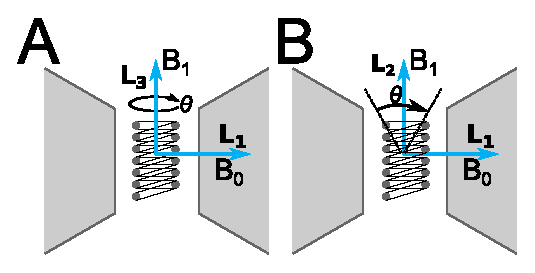
\includegraphics[width=0.5\textwidth]{Kapitel/Ch2-Images/RotateMeLeftRight.eps}
 \caption[Rotation Planes of micro-Helix.]{Shown are the two rotation planes available for crystal rotation in the self-resonant micro-helix of Chapter~5. A) A full 180 degree rotation is available when the ${\textbf B}_1$ is along the L$_3$-axis. B) A second plane is available when the ${\textbf B}_1$ is along the L$_2$-axis. A rotation in this plane is limited by a sinusoidal dependence of the EPR signal. }
 \label{fig:RotateMe}
\end{figure}

\paragraph*{Crystal Rotation} To obtain a magnetic resonance rotation pattern, the crystal must be rotated with respect $\mathbf{B}_0$, illustrated in Fig.~\ref{fig:RotateMe}A. This is currently performed by rotating the entire resonator probe around the L$_3$-axis. If a second plane is needed, the angle can be modified by orientating the $\mathbf{B}_1$ along the L$_2$-axis, illustrated in Fig.~\ref{fig:RotateMe}B by using a 90$^{\circ}$ bend. This secondary plane of rotation is limited since the EPR signal has a sinusoidal dependence is reduced as $\mathbf{B}_1$ becomes parallel to $\mathbf{B}_0$. With a good signal-to-noise ratio, EPR can be collected over a 120 degree rotation.

\section{Finite-element modeling Simulations}
Commercially available electromagnetic finite-modeling software provides a suite in which boundary conditions, sources, and dielectric properties are combined to solve Maxwell's equations in a CAD-like environment. In this dissertation, finite-element modeling is used to design, understand, and optimize microwave resonators. Here, an introduction to Ansys Electromagnetics Suite (Pittsburgh, PA, USA; version 19.4; High Frequency Structure Simulator (HFSS)) and a practical exercise will be developed. 

Ansys HFSS employs ``driven-mode'' and ``eigenmode'' solving domains. The ``eigenmode'' solver uses Maxwell's equations in their variational form to find the lowest energy states of a structure given its boundary conditions and electromagnetic material properties. \cite{sadiku2000numerical,jin2015finite} This lowest energy state, or eigenvalue, is then used to calculate the eigenvectors of the structure, yielding a wave solution. The eigenvalue problem assumes that both the differential equations and the boundary conditions are homogeneous. There is no source exciting the mode of interest. This becomes very important in geometries where the modes of the system are not known. In Ansys Electronics Desktop, solutions are normalized by the electric field (1~V/m) or to the stored electric energy.

The ``driven-mode'' solves the non-homogeneous Maxwell's equations. Practically, one must devise a coupling system in ``driven-mode'' and, in this work, impedance matching considerations are implemented to maximize power transfer to the resonator. The ``driven-mode'' provides outputs similar to a vector network analyzer and is typically normalized to an input power of 1~W. 

\paragraph*{Signal Calculations and Resonator Comparisons.}
A method to obtain the EPR signal has been formulated and is reproduced here. \cite{misrabook} This method uses the fields calculated in Ansys HFSS, accessed by the ``Field Calculator'', to determine a normalized EPR signal under saturating or nonsaturating conditions. This calculation can be performed using eigenmode or driven-mode methods and the scripts for Ansys HFSS are found in Appendix~B.\footnote{All codes and HFSS files can be found at https://github.com/jsidabras/HFSSTutorial/.} 

\begin{wrapfigure}{R}{4cm}
\centering
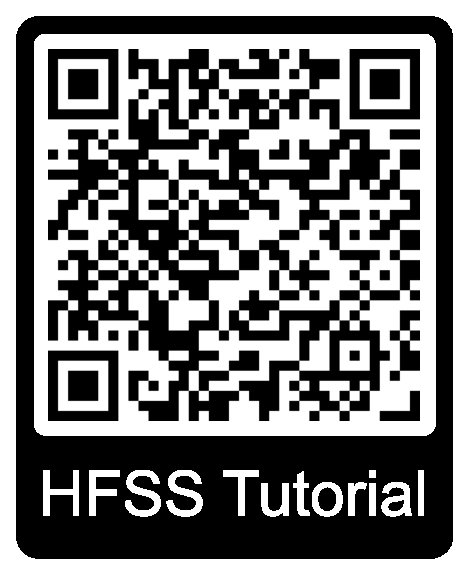
\includegraphics[width=4cm]{Kapitel/Appendix/HFSSTutQR.eps}
\end{wrapfigure}

For a matched reflection cavity and a voltage-sensitive detector, Feher expressed the microwave EPR signal as
\begin{equation}
    S \propto \chi'' \eta Q P^{1/2} \qquad [\text{V}],\label{ch2-fehereq}
\end{equation}
where $\chi''$ is the imaginary part of the magnetic susceptibility which represents the magnitude of the absorption spectrum, $\eta$ is the filling factor, $Q$ is the unloaded $Q_0$-value with a sample, and $P$ is the incident microwave power.  \cite{FeherSignal} The signal is proportional to volts when the system is critically coupled and calculated at microwave resonance. When comparing resonators, the sample has the same concentration for an arbitrary volume and, as such, the magnetic susceptibility $\chi''$ is simply proportional to frequency. This assumption is used to incorporate the Boltzmann factor to resonator comparisons (i.e. temperature or frequency differences).

The $Q$-value of the system can be calculated by the ratio of the stored energy per cycle and the power losses. Such that
\begin{equation}
    Q = \frac{\omega U_m}{P_l},\label{ch2-Qval}
\end{equation}
where $\omega$ is the microwave resonance frequency in radians per second, $U_m$ is the stored magnetic energy, and $P_l$ is the power losses in the cavity walls and sample. At resonance, the magnetic and electric stored energy are equal. \cite{ramo1984fields} However, the magnetic stored energy is chosen for simplicity when dealing with a geometry where there are different dielectric volumes. Electric stored energy includes the relative permittivity $\epsilon_r$ accounted for in each volume, while magnetic stored energy includes the relative permeability $\mu_r$. In this formulation, the relative permeability is equal to unity and only the free-space permeability $\mu_0$ is needed. Therefore the magnetic stored energy is
\begin{equation}
    U_m = \frac{\mu_0}{2} \int \mathbf{H}_1\cdot\mathbf{H}_1^* dV \qquad [\text{W}],
\end{equation}
where ${\textbf H}_1$ is the microwave magnetic field in all space ($V$) including the sample.

The filling factor is defined as the ratio of the magnetic flux density energy in the sample that gives rise to an EPR signal to the microwave magnetic field energy in all space. This can be calculated as
\begin{equation}
 \eta = \frac{\int {\mathbf B}_{1r} \cdot {\mathbf B}_{1r}^* dV_s}{\mu_0 \int {\mathbf H}_1 \cdot {\mathbf H}_1^* dV}, \label{eq-2:filling}
\end{equation}
where ${\textbf B}_{1r}$ is one component of the clockwise (or counter clockwise) rotational component of the linearly polarized flux density ${\textbf B}_1$ perpendicular to the static magnetic field in the sample volume ($V_s$). \cite{jackson1975classical} In magnetic resonance, the spin system is coupled to either the right-handed or left-handed (clockwise or counter clockwise) polarization of the magnetic flux density. \cite{abragam1961}

A linearly polarized wave can be decomposed into two in-phase circular components. From Ref.~[2.\kern-0.4em\citenum{jackson1975classical}], an expression for the right-handed ($+$) or left-handed ($-$) component of the magnetic flux density can be derived, such that
\begin{equation}
    \mathbf{B}_{\pm} =  \mathbf{B}\cdot\frac{\mathbf{\hat{y}} \pm i\mathbf{\hat{z}}}{\sqrt{2}} \qquad \text{[T]}, \label{circpoleHpm}
\end{equation}
where the static magnetic field B$_0$ is in the $\mathbf{\hat{x}}$ direction. In cavity resonators, where the microwave magnetic field is well defined, the left- and right-handed components are equal. However, open structures and systems with multiple wavelengths within the sample could exhibit elliptical polarization. This results in different magnitudes and field profiles for the two components. The component of the magnetic flux density that interacts with the sample during resonance is the amplitude of Eqn.~\ref{circpoleHpm}, therefore, the magnitude of the microwave magnetic flux density in the (right-handed) rotating frame is the amplitude of Re($\mathbf{B}_+\epsilon_+e^{-iwt}$) such that
\begin{equation}
    \mathbf{B}_{1r} =  \frac{|\mathbf{B}_{+}|}{\sqrt{2}} \qquad \text{[T]}. \label{circpoleH}
\end{equation}
Herein, this formulation was only applied to systems that exhibit linear polarization in the sample (Chapter~3 and 5) and other methods were relied upon to approximate the EPR signal in cases where multiple wavelengths are involved (Chapter~4).

The power loss in the system is broken up into two distinct types: dielectric losses and Ohmic losses on the surfaces of conductors. For a bulk conductor, the power dissipated on the surface can be calculated as
\begin{equation}
    P_{lw} = \frac{R_s}{2}\int \mathbf{\hat{n}}\times\mathbf{H}\cdot\mathbf{H}^* dS_w \qquad [\text{W}]
\end{equation}
where $\mathbf{\hat{n}}$ is normal to the conductor surface ($S_w$). The resistance of the surface is calculated by the real part of the surface impedance, defined as
\begin{equation}
    Z_s = \sqrt{\frac{\omega \mu_0}{2 \sigma}}(1-i)
\end{equation}
where $\sigma$ is the conductivity of the metal surface. The power dissipated in a dielectric can be calculated by
\begin{equation}
    P_{ld} = \frac{\omega \epsilon_0 \epsilon_r''}{2}\int \mathbf{E} \cdot \mathbf{E}^* dV_d \qquad [\text{W}],
\end{equation}
where the imaginary part of the dielectric permittivity ($\epsilon_r = \epsilon_r' - i \epsilon_r''$) is integrated over the dielectric volume $V_d$. \cite{jackson1975classical,harrington1961time} The total power loss of the system is the summation of all the power losses of the conductors and $n$ is the number of dielectrics which may include the sample, sample tube, and other plastics and ceramics such that
\begin{equation}
    P_l = P_{lw} + \sum_{i=1}^n P_{ld_i} \qquad \text{[W].}
\end{equation}
The power loss in the system for the sample, resonator walls, and sample holder end sections is defined as $P_s$, $P_w$, and $P_e$, respectively, in the scripts of Appendix~B. The calculations for $P_s$ and $P_e$ rely on the constants \textit{ImDiSam} and \textit{ImDiHold} which are set to the imaginary part of the relative permittivity constant $\epsilon_r''$.

From Eqn.~\ref{ch2-fehereq} the signal can be calculated by substituting the appropriate equations. Two EPR signal conditions can be calculated: signal unsaturable (Su; Unsat.) and signal saturable (Ss; Sat.). In continuous-wave experiments, signal unsaturable is defined as the EPR signal at constant incident power, while signal saturable is defined as the EPR signal at a constant magnetic flux density at the sample. A saturable sample can be calculated by normalizing to the magnetic flux density and computing
\begin{equation}
    S_s = \frac{\chi'' \omega}{10^4 P_l^{1/2} \text{Max}|\mathbf{B}_{1r}|} \int \mathbf{B}_{1r} \cdot \mathbf{B}_{1r}^* dV_s \qquad \text{[V]}. \label{ch2-eq:ss}
\end{equation}{}
The unsaturable sample can be calculated by normalizing to the power and computing
\begin{equation}
    S_u = \frac{\chi'' \omega}{P_l} \int \mathbf{B}_{1r} \cdot \mathbf{B}_{1r}^* dV_s \qquad  \text{[V]}. \label{ch2-eq:su}
\end{equation}{}
The efficiency parameter $\Lambda_{max}$, as introduced by Hyde {\em et al.} \cite{hydehoff}, is defined as
\begin{equation}
    \Lambda_{max} = \frac{1}{10}\frac{\text{Max}|\mathbf{B}_{1r}|}{P_l^{1/2}} \quad \text{[mT/W}^{1/2}], \label{ch2-eq:lammax}
\end{equation}
where Max$|\mathbf{B}_{1r}|$ is the maximum magnitude of $\mathbf{B}_{1r}$ in the sample (typically in the center of the cavity) and is assumed to be uniform over the sample volume. \cite{hydehoff} The scalar converts Gauss into milliTesla. 

To better assess the resonator efficiency when $\mathbf{B}_{1r}$ is not uniform, an average over the sample volume is calculated, 
\begin{equation}
    \Lambda_{ave} = \frac{1}{10}\frac{\int \sqrt{\mathbf{B}_{1r} \cdot \mathbf{B}_{1r}^*} dV_s}{P_l^{1/2} V_t} \quad [mT/W^{1/2}], \label{ch2-eq:lamave}
\end{equation}
where $V_t$ is the total volume of the sample. The average resonator efficiency, which takes into account the $\mathbf{B}_{1r}$ profile along the sample volume, is the measurable value when a nutation experiment is performed.

Finally, the $\Lambda_{ave}$-to-$\Lambda_{max}$ ratio can be used as a metric to quantify the uniformity of the resonator. \cite{UFLGR2017} The B$_1$ profile uniformity (in percent) is defined by 
\begin{equation}
    \Delta B_1 = \frac{\left| \Lambda_{max} - \Lambda_{ave} \right|}{\Lambda_{max}} \times 100\%.
\end{equation}

\section{Experimental Measurement of EPR Spectra}
The EPR experiments performed in this work are as follows:

\subsubsection*{Continuous-wave EPR.}
The continuous-wave (CW) EPR experiment measures the sample using a constant microwave B$_1$ at a fixed frequency ($\omega$) incident on the sample and slowly sweeping B$_0$. As the resonance condition is met, when the incident energy ($E =\hbar \omega$) is equal to the Zeeman splitting, the angular momentum is perturbed and an absorption of the energy is recorded.\footnote{In order to relate this to a real spectrum, we say this happens ``in the neighborhood'' of resonance $\omega_0$ and assume the linewidth is caused by a general broadening from the spin-lattice relaxation time. This assumes homogeneous broadening, as opposed to inhomogeneous broadening. For example, broadening from hyperfine interactions, environmental deviations, etc.}   

At the macro-scale view, the absorption of the microwaves cause a change in the permeability of the sample through a perturbation of the magnetic susceptibility M,
\begin{equation}
    \mu_r(\omega) = \mu_0 (1+M) = \mu_0 (1+ 4 \pi \eta \chi(\omega)), \label{eq-2:permea}
\end{equation} 
where $\eta$ is the filling factor from Eqn.~\ref{eq-2:filling} which describes the flux-linkage efficiency between the applied microwave magnetic field and the sample and $\chi(\omega)$ is the complex time-dependant magnetic susceptibility. For a simple Lorenzian-shaped spectrum, the magnetic susceptibility is 
\begin{equation}
      \chi(\omega) = \frac{(\omega_0 - \omega) T_1 }{1+(\omega_0 - \omega)T_2^2+\gamma^2 H_{1r} T_1 T_2}- i \frac{1}{1+(\omega_0 - \omega)T_2^2+\gamma^2 H_{1r} T_1 T_2}, \label{eq-2:chi}
\end{equation}
where $T_1$ and $T_2$ are the spin-spin and spin-lattice relaxation times, respectively, $\omega_0$ is the frequency of resonance as $\omega$ is swept, $H_{1r}$ is the microwave magnetic field perpendicular to $\vectu{B}{0}$ (Eqn.~\ref{circpoleH} and $\gamma$ is an isotropic gyromagnetic ratio. \cite{abragam1961}

Assuming a simple lumped-circuit resonance consisting of an inductor $L_R$ (which contains the sample) in series with a resistor $R_R$ in parallel with a capacitance $C_R$. The capacitor is chosen so the tank circuit resonates at the frequency $\omega_R^2 L_R C_R = 1$. The detector is placed across the capacitor, measuring the voltage. 

The inductance can be described by
\begin{equation}
    L_R = \mu_r L_0 = \mu_0 (1 + M)L_0 = \mu_0 (1 + 4 \pi \eta \chi)L_0,
\end{equation}
where the permeability of the sample consists of the freespace $\mu_0$ and $4\pi\chi$ is the magnetic susceptibility $M$, modified by the filling factor $\eta$. \cite{ramo1984fields} Although $\chi$ is a function of the incident microwave frequency $\chi(\omega)$, it is omitted for brevity. The resonant tank-circuit resistance and inductance can be further simplified such that
\begin{equation}
    R_R + i \omega L_R = (R_R + 4\pi \omega L_0 \eta \chi'') + i (1+4\pi\eta\chi')\omega L_0
\end{equation}
where $\omega$ is the frequency of operation and resonance occurs in the neighborhood of $(\omega_0-\omega)$. \cite{schumacher1970introduction} The change in magnetic permeability within a resonator is small compared to the microwave inductance and causes only a perturbation in the operating frequency (dispersion; $\chi'$) and losses (absorption; $\chi''$). The resonator impedance is matched to the bridge, called ``critical coupling'', where the phase of the incoming standing-wave voltage cancels the outgoing reflections. At critical coupling, no voltage is detected at the diode. However, in the neighborhood of resonance, the change in the tank-circuit resistance is directly measured as a change in the reflection coefficient. 

In the CW experiment, the static magnetic field is modulated by $B_0 + B_m Cos[2\pi f_m t]$, typically at a modulation frequency $f_m$ of 100~kHz, and is collected using a phase-sensitive detector. \cite{weil2007electron} If the modulation is small, the signal is derivative-like. \cite{Hyde1990pseudo} As the modulation amplitude $B_m$ is increased, the signal increases proportionally until the modulation amplitude approaches the intrinsic line-width of the sample where a broadening occurs. Choosing between signal and signal purity is known as the line-height--line-width compromise and is discussed in Ref.~[2.\kern-0.4em\citenum{eaton2010quantitative}]. 

The modulated reflection coefficient changes are recorded on a detector diode connected to the phase-sensitive detector. When the frequency is held constant, as is typically done with automatic frequency control (AFC), an absorption spectrum is obtained. \cite{poole1967electron} A dispersion signal can be obtained by the frequency control feedback voltage or directly detected by a quadrature microwave channel. Continuous-wave is the standard EPR experiment. 

\subsubsection*{Non-adiabatic and Adiabatic Rapid Scan.}
With modern digital signal processing and fast analog-to-digital converters, the CW experiment has recently been improved upon. The non-adiabatic rapid scan (NARS) \cite{KITTELL2011228, KITTELL201251, KITTELL201568, Hyde2013MDIFF, YU201558} and adiabatic rapid scan (RS) \cite{JOSHI200544,TSEITLIN200948, MITCHELL2012221, RScompare,MOSER2017} methods collect real and imaginary EPR spectra (pure-absorption and pure-dispersion) using magnetic field ($\mathbf{B}_0 + \mathbf{B}_m $) or microwave frequency sweeps without the need for a phase-sensitive detector. Both rapid scan methods produce data that can be post-processed with pseudo-modulation to compare to the conventional first-derivative EPR spectrum using a moving difference (MDIFF) pseudo-modulation. \cite{Hyde2013MDIFF} The non-adiabatic rapid scan (NARS) experiment uses a static field sweep fast enough to overcome $1/f$ noise but remains in thermal equilibrium, while adiabatic rapid scan sweeps the static field fast enough to cause passage. \cite{Weger1960} 

Specifically, the rapid passage regime satisfies the equation
\begin{equation}
    \frac{|\mathbf{B}_{1r}|}{d B_0/dt} \ll \sqrt{T_1 T_2}
\end{equation}
where the magnitude of the magnitude microwave magnetic field $\mathbf{B}_{1r}$, as previously defined in Eqn.~\ref{circpoleH}, and the change in static magnetic field B$_0$ must be much less than the product of the spin-lattice relaxation time $T_1$ and spin-spin relaxation time $T_2$. The adiabatic regime is defined as 
\begin{equation}
    \gamma |\mathbf{B}_{1r}|^2 \gg \frac{d B_0}{dt},
\end{equation}
where $\gamma$ is the the gyromagnetic ratio in MHz/G. Conversely, the non-adiabatic regime is defined as
\begin{equation}
    \gamma |\mathbf{B}_{1r}|^2 \ll \frac{d B_0}{dt}.
\end{equation}
These conditions produce passage. \cite{Weger1960}

The advantage of the non-adiabatic rapid scan experiment is the signal-to-noise improvement of collecting pure-absorption EPR spectra, while adiabatic rapid scan can further improve the continuous-wave and NARS experiment by changing the effective microwave magnetic field at the sample. This allows for an increase of microwave power, and thus, an increase in EPR signal for saturable signals. \cite{JOSHI200544} It should be noted that the excitation of a spin packet goes through a continuum of passage from the steady-state CW experiment to the non-adiabatic rapid scan to adiabatic rapid scan, and finally to the free-induction decay pulse. 

While the non-adiabatic rapid scan method can be implemented on commercial pulse bridges with no hardware changes, it does require some technical expertise. \cite{MOSER2017} However, to perform adiabatic rapid scan experiments on protein samples, custom current drivers are needed to increase the swept field amplitude. For simplicity, in this work, only the non-adiabatic rapid scan experiment has been implemented.

\subsubsection*{Electron Spin Echo Pulse.}
The field-swept two-pulse electron spin-echo (ESE) experiment uses a ${\pi/2\!-\!\tau\!-\!\pi}$ pulse sequence. A $\pi/2$-pulse is defined as enough microwave power to tip the magnetization of a spin packet into the M$_x$-M$_y$ plane. Such a pulse is applied Over a time $\tau$, the magnetization dephases into the $x$-$y$-plane, where an applied $\pi$-pulse inverts the magnetization. After $\tau$ seconds the spin packet becomes coherent and an echo is formed. The echo is recorded, where the intensity is a function of the magnetic susceptibility absorption $\chi''$ (Eqn.~\ref{eq-2:chi}) interacting with the resonator. The echo is proportional to the absorption of the spins at a single static field position. The static field is stepped and a whole spectrum is acquired. \cite{schweiger2001principles} For systems with little nuclei interaction, the ESE experiment will mimic the pure absorption spectrum of the CW experiment. This is the standard pulse sequence to collect an EPR spectrum, and the pulse sequence is illustrated in Fig.~\ref{fig:EPRpulse}.

\begin{figure}[ht]
 \centering
 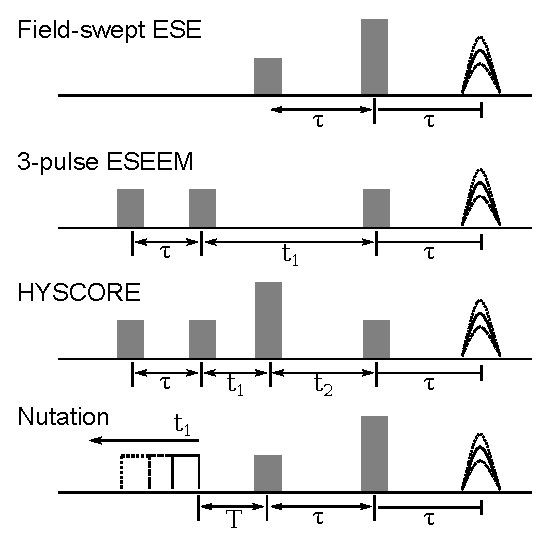
\includegraphics{Kapitel/Ch1-images/PulseExperiments.eps}
 \caption[Pulse EPR sequences.]{The pulse EPR sequences used in this work. Field-swept electron spin echo (ESE) is performed over a series of field steps, recording the entire spectrum. Electron Spin Echo Envelope Modulation (ESEEM) and Hyperfine Sub-level Correlation (HYSCORE) are performed at a single field position. The nutation experiment is used in this work to determine the efficiency parameter $\Lambda_{ave}$. }
 \label{fig:EPRpulse}
\end{figure}

Specifically, the signal from a microwave pulse is derived from the reciprocity principle of electromagnetics. \cite{HOULT2011329} The initial magnitude of the magnetization can be described as $\mathbf{M} = M_0 \mathbf{B}_z$, where $M_0$ is the dc bulk magnetization. When $\mathbf{B}_{1r}$ is applied, the bulk magnetization takes the form of the magnetic susceptibility of Eqn.~\ref{eq-2:chi}. If the excitation coil is the same as the pickup coil, after a $\pi/2$-pulse is applied, and electromotive force (emf) is induced on the coil such that 
\begin{equation}
    \xi = - \int \frac{\partial \mathbf{B}_{1r} \cdot \mathbf{M}}{\partial t} dV_s,
\end{equation}
which is transferred to a voltage across the tank-circuit capacitance. The voltage, assuming a homogeneous $\mathbf{B}_{1r}$ and a unit volume, is such that
\begin{equation}
    V_0 = - 4\pi \eta \int \frac{\partial \mathbf{B}_{1r} \cdot \mathbf{M}}{\partial t} dV_s = - 4 \pi \eta \frac{\partial \phi}{\partial t},
\end{equation}
where $\partial \phi/\partial t$ is the time-varying magnetic flux, which includes the permeability defined in Eqn.~\ref{eq-2:permea}. \cite{schumacher1970introduction,slichter1978principles,HOULT2011329} The final output to the receiver is multiplied by the $Q$-value of the tank circuit, which transforms the voltage proportional to the stored energy of the circuit. \cite{ramo1984fields} The formulation of $V_0 Q$ can be related directly to the parameters defined by Feher in Eqn.~\ref{ch2-fehereq}, where the applied microwave magnetic field is held constant in order to provide a $\pi/2$-pulse, as defined by the saturable signal conditions of Eqn.~\ref{ch2-eq:ss}.

The voltage $V_0$ decays exponentially with the spin-lattice relaxation time $T_2$ and, within the decay envelope, exists the magnetization dephasing from the $x$-$y$-plane. The signal directly after a $\pi/2$-pulse is known as the free induction decay (FID) and it is this dephasing that is refocused after time $\tau$ to form the echo in the ESE experiment. Therefore, the experimental parameter $\tau$ must be chosen to allow for sufficient ring-down of the tank-circuit, but not so long as the signal $V_0$ has decayed beyond detection.

\subsubsection*{ESEEM and HYSCORE.}
The Electron spin echo envelope modulation (ESEEM) experiment has a  pulse sequence of ${\pi/2\!-\!\tau\!-\!\pi/2\!-\!t_1\!-\!\pi/2}$. The three-pulse variation of ESEEM (3P-ESEEM) puls sequence is illustrated in Fig.~\ref{fig:EPRpulse}. ESEEM is capable of resolving hyperfine and quadrupole interactions of the electron to neighboring nuclei. It is complementary to electron-nuclear double resonance experiments (ENDOR). \cite{schweiger2001principles,Doorslaer2007,Harmer2009,CUTSAIL20151370}

The 3P-ESEEM signal used in this work arises from the semi-forbidden transitions between the different $M_s$ manifolds ($\pm \ket{\frac{1}{2}}$; Fig.~\ref{fig:EPREnergy}), but within the same $M_I$ manifold. This nuclear coherence mixing is directly probed by the dephasing that is occurring at time $\tau$ which is allowed to mix for time $t_1$. 

Unlike the two-pulse ESEEM signal, the 3P-ESEEM does not obtain the sum and differences of the modulating frequencies, potentially simplifying analysis. However, a drawback of the 3P-ESEEM method is the dependence of the signal on the $\tau$ chosen. Known as ``$\tau$-suppression'' occurs because of the time at which the coherence mixing $\pi/2$-pulse starts could be at a null of the nuclear modulation frequency. \cite{schweiger2001principles} This effect can be minimized by summing a series of 3P-ESEEM measurements at different $\tau$ values.

Two regimes of hyperfine coupling exist, denoted as strong $a_{iso}/2 < \nu_n$ and weak $a_{iso}/2 > \nu_n$ coupling, depicted in the bottom-right inset of Fig.~\ref{fig:EPREnergy}. The modulating resonance frequency $\nu_n$ is related to the nuclei by the nuclear Zeeman energy $-g_n \beta_n B_0/\hbar$. The tensor information is directly observed from the summation of the hyperfine and quadrupole interactions of Eqns.~\ref{eq-2:hfi} and \ref{eq-2:nqi}. Using an ESEEM experiments, the modulation frequencies $2\nu_n \pm 3P_z$ for strong coupling and $a_{iso} \pm 3P_z$ for weak coupling (Fig.~\ref{fig:EPREnergy} $\mathbf{d}$, $\mathbf{e}$, $\mathbf{f}$, $\mathbf{g}$) are directly observed. In addition, the double-quantum peaks (Fig.~\ref{fig:EPREnergy} $\mathbf{h}$, $\mathbf{i}$) are observed at the frequencies $\nu^DQ_{\alpha,\beta}$ described by Eqn.~\ref{eq-2:doubleQ}. The modulation depth observed in the time-domain trace is dictated by
\begin{equation}
    k(\theta) = \text{Sin}^2(2\theta) = \bigg(\frac{B_\theta}{\nu_I}{\nu_\alpha \nu_\beta}\bigg)^2
\end{equation}
where $\theta$ is the angle between the non-isotropic electron-nuclear hyperfine tensor $\mathbf{T}$ of Eqn.~\ref{eq-2:hfiT} and the static magnetic field $\mathbf{B}_z$. When either $\mathbf{T}$ is zero or $\mathbf{B}_z$ is aligned with a principal axis, the modulation depth is reduced to zero.

The hyperfine sublevel correlation (HYSCORE) experiments add an additional pulse to the 3-Pulse ESEEM. A  ${\pi/2\!-\!\tau\!-\!\pi/2\!-\!t_1\!-\!\pi\!-\!t_2\!-\!\pi/2}$ pulse sequence results in an echo $\tau$ seconds after the last $\pi/2$ pulse. The values for $t_1$ and $t_2$ are swept to form a 2D experiment at a fixed static magnetic field position. The HYSCORE experiment allows for the separation of overlapping modulation frequencies found in large anisotropic hyperfine systems. Additionally, HYSCORE separates the strong $a_{iso}/2 < \nu_n$ and weak $a_{iso}/2 > \nu_n$ coupling regimes into the ($-$,$+$) quadrant and ($+$,$+$), respectively. The use of HYSCORE allows for a visual representation of the different modulating frequencies such that the $\nu_n$ or $a_{iso}/2$ can be read directly from the graph. 

Although HYSCORE is a useful tool for visualization and human-aided analysis, a set of ESEEM spectra are typically simulated for fitting and following orientation dependant single crystal data to obtain the full hyperfine-tensor. \cite{Shane1994SingleCrystalESEEM}

\subsubsection*{Nutation.}
The nutation experiment is performed at a field position of maximum EPR signal and a perturbation pulse is added to the electron spin-echo experiment such that a pulse sequence of ${t_1\text{-pulse}\!-\!\text{T}\!-\!\pi/2\!-\!\tau\!-\!\pi}$ if formed. The $t_1$-pulse is varied resulting in a perturbation on the electron spin echo experiment at a fixed field. The variation is a function of the tip angle of the spin-system and can be related to the microwave magnetic field $\mathbf{B}_1$ incident on the sample. In resonators with inhomogeneous fields, the average of $\mathbf{B}_{1r}$ is measured and is directly comparable to $\Lambda_{ave}$ of Eqn.~\ref{ch2-eq:lamave}.

The Rabi oscillation frequency $f_{rab}$ produced in a nutation experiment can be determined by
\begin{equation}
  f_{rab} = \frac{\gamma B_{1r}}{2 \pi },
\end{equation}
where $\gamma$ is the gyromagnetic ratio and B$_{1r}$ is the magnetic flux density incident on a sample. When measuring B$_{1r}$, the average over the entire sample is observed. If the incident $\mathbf{B}_1r$ was homogeneous, a single frequency would be produced. However, for cavities with non-uniform $\mathbf{B}_1r$ a distribution of frequencies is generated and can be assessed by the Fourier transform of the Rabi oscillations. 

{\renewcommand{\bibsection}{\clearpage\section*{\bibname}\markboth{\bibname}{\bibname}}
\renewcommand{\bibname}{CHAPTER 2. REFERENCES}
\bibliographystyle{elsarticle-num}
\bibliography{Kapitel/Ch5-References}
}

